\documentclass[a4paper, 11pt]{article}

\setlength\parindent{0pt}

\usepackage[ngerman]{babel}
\usepackage[utf8]{inputenc}

\usepackage{amsfonts}
\usepackage{amsmath}
\usepackage{cancel}
\usepackage{graphicx}
\usepackage{mathcomp}

\usepackage[top=3.0cm, bottom=3.0cm, left=2.0cm, right=2.0cm]{geometry}

\usepackage{fancyhdr}
\pagestyle{fancy}

\lhead[]{Machine Learning 1 — WS2011 — Module IN2064}	\chead[]{}	\rhead[]{Project Script · Page \thepage}

\lfoot[]{\hrule}	\cfoot[]{}	\rfoot[]{}

\begin{document}

\begin{center}
	Daniel Hein · M.-Nr. 03627602
\end{center}

\section{Data Preprocessing}
To extract relevant features from the images preprocessing is necessary. To do so we created a preprocessing pipeline that consists of five separate functions.
\newline

\textbf{Sharpest image.} 
\newline
\newline
INPUT: grayscale image matrix $I$
\newline
OUTPUT: estimated sharpness $s$
\newline
VARIABLES TO ADJUST: -
\newline
\newline
\begin{center}\includegraphics[width=80mm]{c2_o.png}\includegraphics[width=80mm]{l1_o.png}
\end{center}
Each image stack consists between around 8 and 18 photography’s of the same part of one worm. The images differ only in the focal plane that is shown. In the most cases only one of these images shows the mitochondria in a sharp and clear way that can be used to classify the mitochondria. The manual process is to look at each of the images, select the sharpest and proceed with the next classification tasks only with this one. If a program should become able to classify automatically, it is necessary to find a way to select the sharpest image automatically, too. 
\newline
For this purpose a simple gradient based estimation function is used. The grayscale image is represented by the matrix $I\subseteq{\mathbb N}^{m \times n}$ with values in the range $[0,255]$ with 0 for black and 255 for white pixels. The sum over the gradients $I_x$ and $I_y$ in both image dimensions $x$ and $y$ normalized by the number of gradients gives a good estimation on how sharp a photography actually is. 

\begin{equation}
	I_x = \frac{\partial I}{\partial x} \qquad I_y = \frac{\partial I}{\partial y}
\end{equation}

\begin{equation}
	s = \frac{\sum_{i=1}^{m}\sum_{j=1}^{n}S_{ij}}{mn} 
\end{equation}

\begin{equation}
	S_{ij}=\sqrt{({{I_x}_{ij}}^2+{{I_y}_{ij}}^2)}
\end{equation}


The higher the value $s$ the sharper the image. A disadvantage of this simple method is that one usually  can only compare images showing the same motive and so in real image processing software much better methods for estimating image sharpness are in use. Nevertheless it has shown to be a sufficient method for our purposes. Because we are only comparing images within on single stack and they all show the exact same microscope photography.
\newline
\newline

\textbf{Reduced noise.} 
\newline
\newline
INPUT: grayscale image matrix $I$
\newline
OUTPUT: grayscale image matrix $I$
\newline
VARIABLES TO ADJUST: neighborhoods of size $m$-by-$n$ to estimate the local image mean and standard deviation
\newline
\newline
Due to the microscope environment the pictures are noisy. One reason is for example the sensor of the build-in camera. Reducing the noise will improve finding mitochondria in the images. We decided to use a pixelwise adaptive Wiener method based on statistics estimated from a local neighborhood of each pixel. For this reason the value 3 for $m$ and $n$ has proven convenient.
\newline
\newline

\textbf{Histogram and image contrast.} 
\newline
\newline
INPUT: grayscale image matrix $I$
\newline
OUTPUT: grayscale image matrix $I$
\newline
VARIABLES TO ADJUST: $\alpha$ and $\beta$ representing percentages of how many pixels in $I$ become black and how many become white
\newline
\newline
\begin{center}\includegraphics[width=80mm]{c2_ad.png}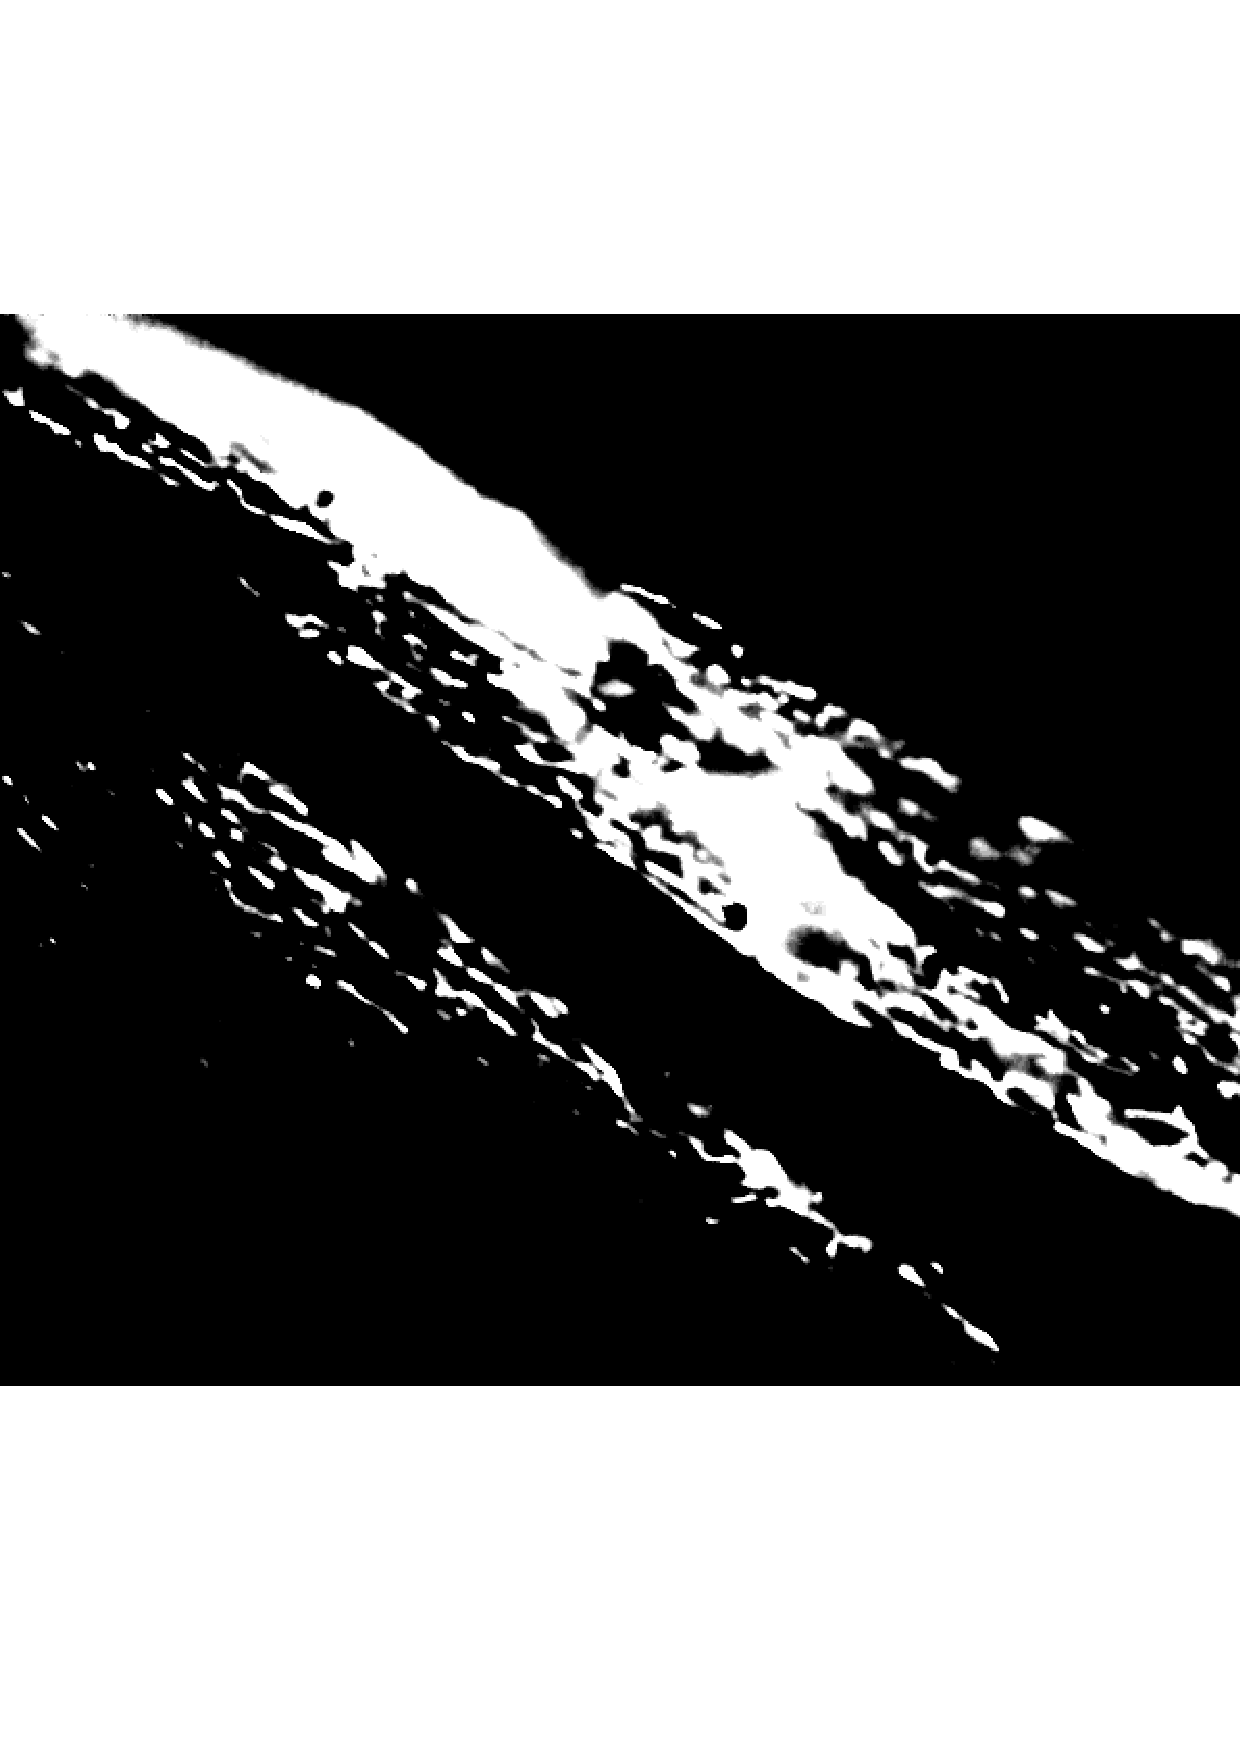
\includegraphics[width=80mm]{l1_ad.png}
\end{center}
\begin{center}\includegraphics[width=80mm]{c2_hist.png}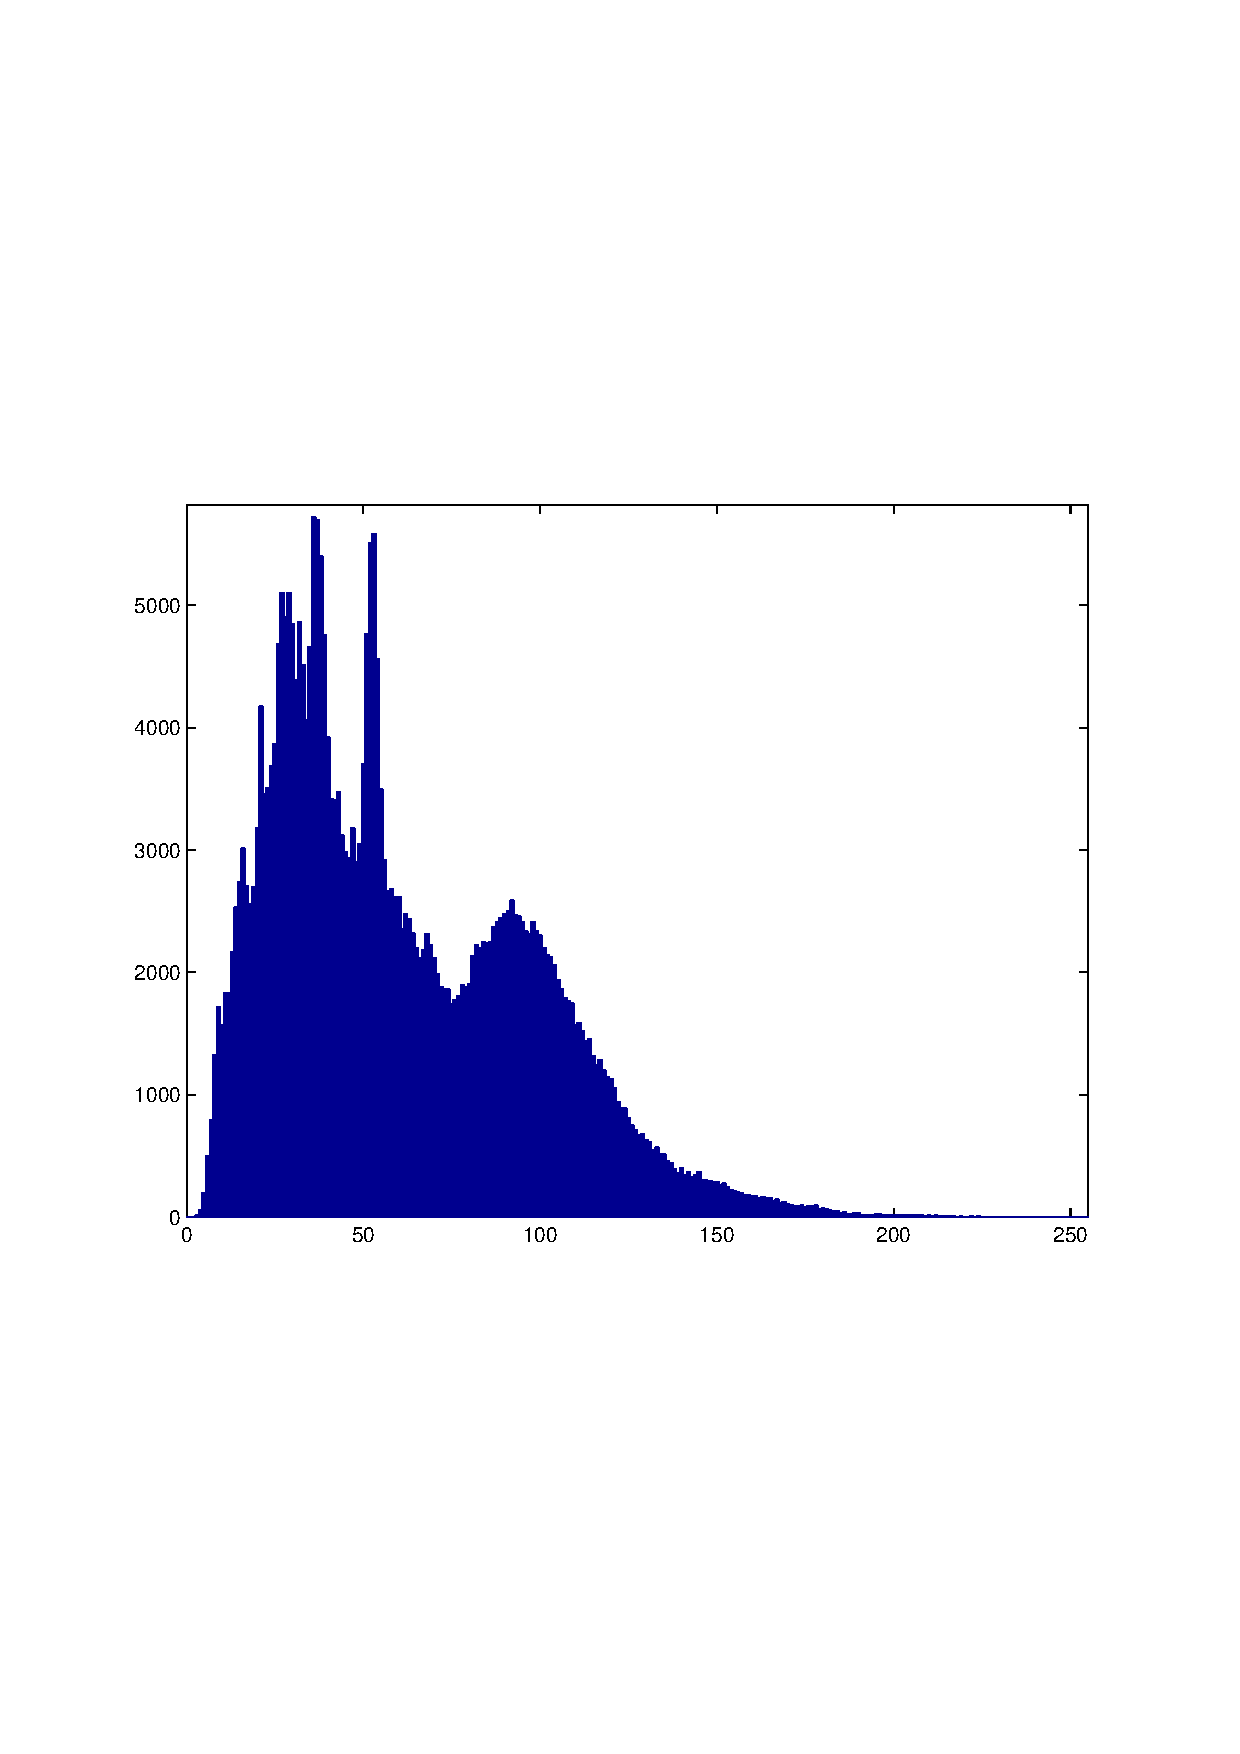
\includegraphics[width=80mm]{l1_hist.png}
\end{center}
To adjust the optimal contrast of each image it is necessary to have a look on the histograms and how the different levels (0 to 255) of gray are distributed all over one image. The task is to find suitable values for $b_{l}$ the lower bound below which everything goes to 0 (black) and the $b_u$ the upper bound above which everything goes to 255 (white). 

\begin{equation}
	f_l(l)=\sum_{i=1}^{l}h_i\leq\beta\sum_{i=1}^{256}h_i \qquad f_u(u)=\sum_{i=1}^{u}h_{256-i+1}\leq\alpha\sum_{i=1}^{256}h_i
\end{equation}

\begin{equation}
	1 \leq l \leq 256 \qquad 1 \leq u \leq 256
\end{equation}

\begin{equation}
	b_l=\frac{\mbox{argmax}_b(f_B)}{256} \qquad b_u=\frac{\mbox{argmax}_u(f_u)}{256}
\end{equation}

\begin{equation}
	\alpha + \beta \leq 1
\end{equation}

The gray scale levels in between are scaled to fit into the histogram of the output image. The result is a high contrast image in which mitochondria are much easier to find.
Because of all the images have different histograms it is not possible to use the same lower bound and upper bound for all of them. So we defined the new variables black percentage and white percentage corresponding to how many of the pixels should become 0 (black) or 255 (white) after the adjustment. Using this procedure we are able to find the optimal bounds for each individual image. The performance of the later classification process will highly depend on the output quality of this contrast adjustment. In order to find the best values for the variables black percentage and white percentage we used the optimization tools of MatLab. The variables to optimize for are black percentage and white percentage and the error to minimize is the misclassification rate on the training set. 
\newline
\newline

\textbf{Binary image.} 
\newline
\newline
INPUT: grayscale image matrix $I$
\newline
OUTPUT: binary image matrix $I_bw$
\newline
VARIABLES TO ADJUST: level above which all pixels become white and below which all pixels become black
\newline
\newline
\begin{center}\includegraphics[width=80mm]{c2.png}\includegraphics[width=80mm]{l1.png}
\end{center}
After improving the contrast of each image it can easily be converted to a binary image in that the mitochondria can be found as white areas.
\newline
\newline

\textbf{Boundaries.} 
\newline
\newline
INPUT: binary image matrix $I_bw$
\newline
OUTPUT: vector $b$ containing mitochondria boundaries
\newline
VARIABLES TO ADJUST: values of pixels below and above that a boundary is not describing valid mitochondria
\newline
\newline
\begin{center}\includegraphics[width=80mm]{c2_m.png}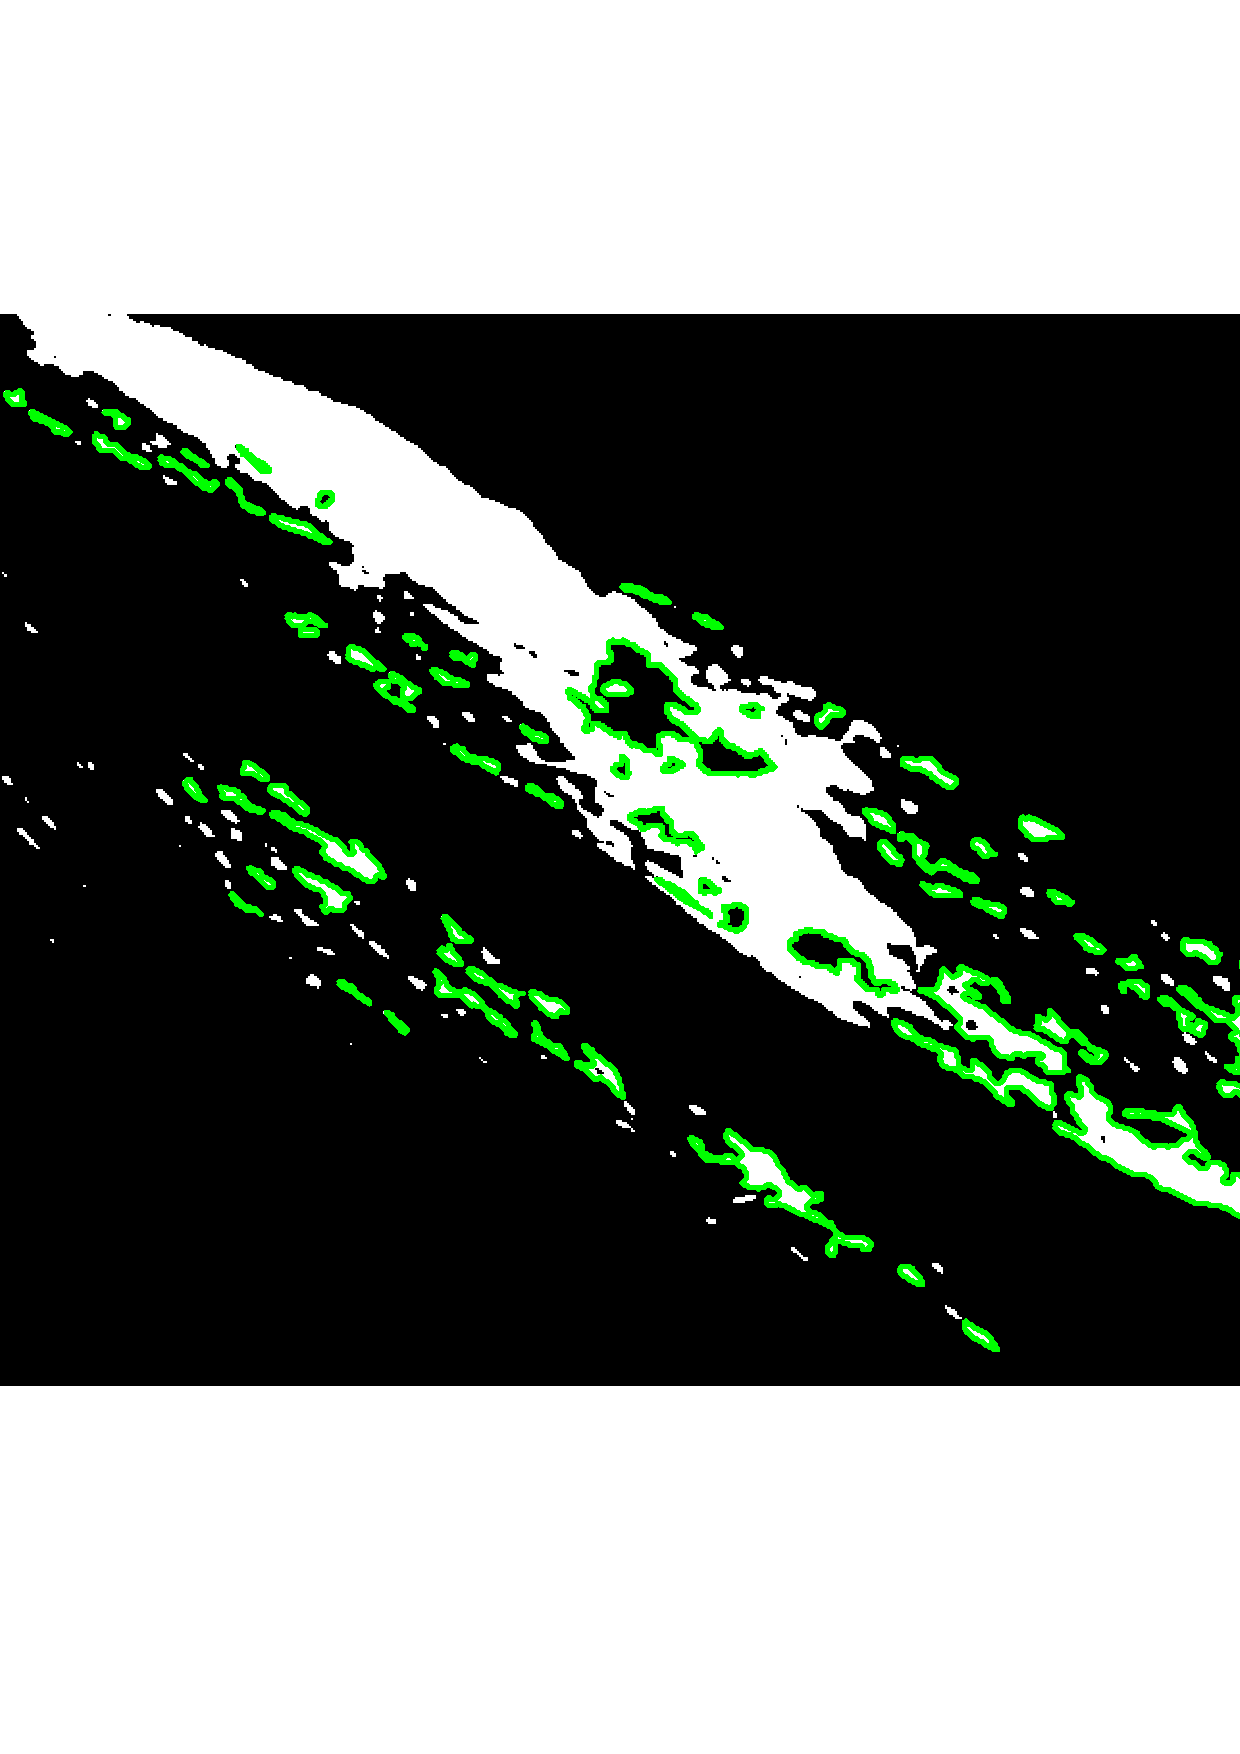
\includegraphics[width=80mm]{l1_m.png}
\end{center}
Using a standard MatLab function it is possible to trace the exterior boundaries of the mitochondria in the binary image. After filtering out objects that are to big or to small to be valid mitochondria we have generated a set of vectors each containing the borders of one of the mitochondria.
\end{document}